\documentclass[UTF8,a4paper,12pt]{ctexart}

\usepackage{geometry}
\usepackage{booktabs}
\usepackage{array}
\usepackage{xcolor}
\usepackage{listings}
\usepackage{amsmath}
\usepackage{graphicx}
\usepackage{float}
\usepackage{hyperref}

\geometry{left=2.5cm,right=2.5cm,top=2.5cm,bottom=2.5cm}
\hypersetup{
    colorlinks=true,
    linkcolor=black,
    urlcolor=blue
}

\lstdefinestyle{cppstyle}{
    language=C++,
    basicstyle=\ttfamily\small,
    keywordstyle=\color{blue!70!black},
    commentstyle=\color{green!40!black},
    stringstyle=\color{red!60!black},
    numbers=left,
    numberstyle=\tiny\color{gray},
    stepnumber=1,
    numbersep=8pt,
    frame=single,
    breaklines=true,
    columns=fullflexible,
    tabsize=4,
    showstringspaces=false
}

\title{并行程序设计 Lab2 SIMD 编程实验报告\\口令猜测中的 MD5 SIMD 加速}
\author{姓名：刘蔚霖 \quad 学号：2412727}
\date{\today}

\begin{document}
\pagenumbering{gobble}
\maketitle
\thispagestyle{empty}
\tableofcontents
\thispagestyle{empty}
\newpage
\pagenumbering{arabic}
\setcounter{page}{1}
\pagestyle{plain}

\begin{abstract}
本实验选择口令猜测任务中的 MD5 哈希阶段作为 SIMD 加速对象，在 ARM OpenEuler 服务器上使用 NEON Intrinsics 实现 4 路并行 MD5。
本文先说明 4 路 NEON 并行的实现方式和优化细节，再验证串行 MD5 与 SIMD MD5 的正确性，随后比较 \texttt{-O0}/\texttt{-O1}/\texttt{-O2} 下的加速比，并使用 \texttt{perf stat}、\texttt{perf report} 和反汇编分析性能瓶颈。当前 SIMD 版本在 \texttt{-O1}/\texttt{-O2} 下的 Hash 阶段加速比分别为 2.61x 和 2.74x，已达到 2.0x 以上要求。
\end{abstract}

\noindent\textbf{代码仓库：}\url{https://github.com/Aokiuuz/nku_parallel.git}

\section{实验环境与评价指标}

\subsection{实验环境}

实验平台为 ARM OpenEuler 服务器，目标指令集为 AArch64，SIMD 扩展为 ARM NEON。代码使用 C++ 实现，串行版本调用标量 \texttt{MD5Hash}，并行版本调用 \path{MD5Hash_simdversion}。性能采集工具包括 \texttt{perf stat}、\texttt{perf record}、\texttt{perf report} 和 \texttt{objdump}。为避免单次运行波动，所有 \texttt{perf stat} 和运行时间均采用 3 次重复运行的平均值。

\begin{table}[H]
    \centering
    \caption{实验环境}
    \begin{tabular}{ll}
        \toprule
        项目 & 配置 \\
        \midrule
        运行平台 & ARM OpenEuler 服务器 \\
        处理器架构 & AArch64 \\
        SIMD 扩展 & ARM NEON，128-bit 向量寄存器 \\
        编程语言 & C++，NEON Intrinsics \\
        编译选项 & \texttt{-O0}、\texttt{-O1}、\texttt{-O2} \\
        性能工具 & \texttt{perf stat}、\texttt{perf record/report}、\texttt{objdump} \\
        测试数据 & 口令训练集与候选口令生成结果，候选规模约 $10^7$ \\
        \bottomrule
    \end{tabular}
\end{table}

\subsection{实验流程}

实验流程分为五步。第一，设计算法，确定将 4 个独立候选口令映射到 NEON 的 4 个 32-bit lane 中并行执行 MD5。第二，分别编译串行版本和 SIMD 版本，并在 \texttt{-O0}/\texttt{-O1}/\texttt{-O2} 三种优化等级下生成独立可执行文件。第三，运行正确性测试，比较 SIMD 每个 lane 的输出与串行 MD5 输出是否一致。第四，记录 Hash 阶段运行时间，计算 Hash 加速比。第五，使用 perf 统计硬件计数器，并对 SIMD 版本进行采样和反汇编分析。

\begin{lstlisting}[style=cppstyle,caption={实验采集流程},language=bash]
# 1. 设计算法：4 路 NEON SIMD 并行 MD5

# 2. 编译 O0/O1/O2 版本
g++ -std=c++11 -O0 *.cpp -o main_O0
g++ -std=c++11 -O1 *.cpp -o main_O1
g++ -std=c++11 -O2 *.cpp -o main_O2

# 3. 运行正确性测试并记录输出
./main_O2 > data/perf_results/O2_simd_run.out

# 4. 采集 Hash time 并计算 Hash 加速比

# 5. 采集 perf stat、热点和反汇编
perf stat -r 3 -e cycles,instructions,branch-misses,cache-references,cache-misses ./main_O2
perf record -g ./main_O2
perf report --stdio > data/perf_results/O2_simd_report.txt
objdump -d ./main_O2 > data/perf_results/O2_simd_main.asm
\end{lstlisting}

\subsection{评价指标}

本文主要使用 Hash 加速比。Hash 加速比只比较 MD5 计算阶段，能够直接反映 SIMD 化对哈希函数本身的优化效果：

\[
S_{\text{hash}}=\frac{T_{\text{hash, serial}}}{T_{\text{hash, SIMD}}}.
\]

训练阶段 \texttt{Train time} 和候选生成阶段 \texttt{Guess time} 不参与加速比计算，因为训练和候选生成不是本次 SIMD 优化目标；但在整程序 perf 分析中仍保留这些阶段，用于解释完整程序热点分布。

\section{算法迭代设计：为什么能加速（基础要求）}

\subsection{数据级并行思路}

口令猜测程序由 PCFG 模型训练、候选口令生成和 MD5 哈希三个主要阶段组成。候选生成阶段维护优先队列并产生字符串，哈希阶段对大量独立候选口令计算 MD5。由于不同口令之间的 MD5 计算互不依赖，且 MD5 的 64 轮计算主要由 32 位整数加法、位运算和循环左移组成，适合使用 SIMD 指令进行数据级并行。

MD5 对每个 512-bit 消息块执行 64 轮迭代，内部维护 4 个 32-bit 状态字 $A,B,C,D$。每一轮的输入包括当前状态、一个 message word、一个常量和一个循环左移位数。对单个口令而言，这 64 轮之间存在严格的数据依赖，不能简单把同一个口令的 64 轮拆开并行；但不同口令之间完全独立，因此可以把“口令维度”作为并行维度。也就是说，SIMD 并不是并行化同一个 MD5 的轮次，而是同时执行 4 个 MD5。

本实验的核心思想是将 4 个候选口令分别放入 NEON 向量的 4 个 lane 中。MD5 状态变量 $A,B,C,D$ 从标量 \texttt{bit32} 改为 \texttt{uint32x4\_t}，每个 lane 对应一个口令。这样一次 SIMD 调用可同步处理 4 个口令：

\[
\begin{aligned}
A &= (A_0,A_1,A_2,A_3),\\
B &= (B_0,B_1,B_2,B_3),\\
C &= (C_0,C_1,C_2,C_3),\\
D &= (D_0,D_1,D_2,D_3).
\end{aligned}
\]

对于 MD5 中的 F/G/H/I、FF/GG/HH/II 轮函数，标量位运算被替换为 NEON 的 \texttt{vandq\_u32}、\texttt{vorrq\_u32}、\texttt{veorq\_u32}、\texttt{vaddq\_u32} 等向量操作。每轮的数学含义不变，只是同时作用于 4 个 lane。

\begin{table}[H]
    \centering
    \caption{标量 MD5 到 NEON SIMD 的映射}
    \begin{tabular}{lll}
        \toprule
        标量操作 & NEON 操作 & 作用 \\
        \midrule
        \texttt{x + y} & \texttt{vaddq\_u32(x, y)} & 4 个 lane 同时做 32-bit 加法 \\
        \texttt{x \& y} & \texttt{vandq\_u32(x, y)} & 4 个 lane 同时做按位与 \\
        \texttt{x | y} & \texttt{vorrq\_u32(x, y)} & 4 个 lane 同时做按位或 \\
        \texttt{x \textasciicircum{} y} & \texttt{veorq\_u32(x, y)} & 4 个 lane 同时做按位异或 \\
        \texttt{\~{}x} & \texttt{vmvnq\_u32(x)} & 4 个 lane 同时取反 \\
        循环左移 & \texttt{vshlq\_n\_u32}/\texttt{vshrq\_n\_u32} & 常量移位后合并 \\
        \bottomrule
    \end{tabular}
\end{table}

因此，理论上一次 SIMD 调用能覆盖 4 个候选口令的 MD5 计算。如果忽略装载、padding、尾部处理和寄存器调度开销，Hash 阶段的理想上限接近 4x。实际测得 \texttt{-O1}/\texttt{-O2} 下为 2.61x 和 2.74x，说明主要收益来自 4 路数据并行，但仍受到消息预处理、内存访问和编译器生成代码质量的限制。

\subsection{关键代码}

SIMD 版本的接口如下：

\begin{lstlisting}[style=cppstyle,caption={SIMD MD5 接口}]
void MD5Hash(const string &input, bit32 *state);
void MD5Hash_simdversion(const string input[4], uint32x4_t state[4]);
\end{lstlisting}

SIMD 版本的基本轮函数将标量宏改写为 NEON 运算。例如：

\begin{lstlisting}[style=cppstyle,caption={NEON 轮函数}]
#define F_SIMD(x, y, z) \
    (vorrq_u32(vandq_u32((x), (y)), vandq_u32(vmvnq_u32((x)), (z))))

#define ROTATELEFT_SIMD(num, n) \
    (vorrq_u32(vshlq_n_u32((num), (n)), vshrq_n_u32((num), 32 - (n))))

#define FF_SIMD(a, b, c, d, x, s, ac) \
    do { \
        (a) = vaddq_u32((a), \
              vaddq_u32(F_SIMD((b), (c), (d)), \
              vaddq_u32((x), vdupq_n_u32(ac)))); \
        (a) = ROTATELEFT_SIMD((a), (s)); \
        (a) = vaddq_u32((a), (b)); \
    } while (0)
\end{lstlisting}

在主程序中，每当候选口令积累到一定规模后，将其按 4 个一组送入 SIMD MD5。若剩余口令不足 4 个，则继续用串行 MD5 处理，避免越界。

\begin{lstlisting}[style=cppstyle,caption={main.cpp 中的批量哈希}]
uint32x4_t state[4];
size_t i = 0;
for (; i + 3 < guesses.size(); i += 4)
{
    MD5Hash_simdversion(&guesses[i], state);
}

bit32 tail_state[4];
for (; i < guesses.size(); i += 1)
{
    MD5Hash(guesses[i], tail_state);
}
\end{lstlisting}

\subsection{降低额外开销的实现细节}

\path{guess_2} （具体代码详见github库）是从标量 MD5 到 SIMD MD5 的初改版，关键改动是先把并行维度确定为“口令维度”。标量版本一次只维护一组 $A,B,C,D$ 状态，\path{guess_2} 则把状态改为 \texttt{uint32x4\_t}，让 4 个 lane 分别保存 4 个候选口令的状态；同时把 MD5 的 F/G/H/I 逻辑函数和 FF/GG/HH/II 轮函数改写为 NEON Intrinsics，用 \texttt{vaddq\_u32}、\texttt{vandq\_u32}、\texttt{vorrq\_u32}、\texttt{veorq\_u32} 等向量指令同步完成 4 份 MD5 计算。主程序也相应改为每 4 个候选口令组成一批调用 \texttt{MD5Hash\_simdversion}，尾部不足 4 个的口令仍由串行 \texttt{MD5Hash} 处理。这个版本已经体现了 SIMD 的核心收益：同一条向量指令同时服务 4 个互不依赖的口令。

从 \path{guess_2} 初改版到当前版本，算法迭代的核心是减少 SIMD 计算前后的额外开销。初改版仍保留了较多标量程序的组织方式，例如每 4 个口令先构造临时 \texttt{string[4]}，每个 lane 分别调用 \texttt{StringProcess} 做动态 padding，SIMD 轮函数以普通函数形式调用，循环左移也使用变量移位实现。这些操作不属于 MD5 核心轮函数，却会在大量候选口令上反复发生，抵消一部分 4 路并行收益。当前版本在此基础上继续迭代：直接传入连续字符串地址，减少口令批量打包复制；将短口令单块 padding 改为栈上构造 message word，减少 \texttt{new/delete} 和内存初始化；把轮函数展开并使用常量移位指令，降低函数调用与移位控制开销。因此，当前版本的加速来自两部分叠加：一是 4 个独立 MD5 的数据级并行，二是减少 SIMD 外围的字符串、padding 和函数调用成本。

\subsubsection{减少字符串复制}

原始批量哈希写法中每 4 个口令会构造一次 \texttt{pw\_batch}，这会触发 4 次字符串拷贝。当前写法将 SIMD 函数接口改为接收连续字符串地址，主程序直接传入候选口令数组中的当前位置：

\begin{lstlisting}[style=cppstyle,caption={避免 string 批量复制}]
void MD5Hash(const string &input, bit32 *state);
void MD5Hash_simdversion(const string input[4], uint32x4_t state[4]);

static void HashGuessesSimd(const vector<string> &guesses)
{
    uint32x4_t state[4];
    size_t i = 0;
    for (; i + 3 < guesses.size(); i += 4)
    {
        MD5Hash_simdversion(&guesses[i], state);
    }

    bit32 tail_state[4];
    for (; i < guesses.size(); i += 1)
    {
        MD5Hash(guesses[i], tail_state);
    }
}
\end{lstlisting}

\subsubsection{将 SIMD 轮函数宏展开}

函数式写法中 \texttt{F\_simd}、\texttt{FF\_simd} 等为普通函数。在 \texttt{-O0} 下编译器通常不会内联这些函数，MD5 的 64 轮计算会产生大量函数调用开销。当前写法将其改为宏展开，使 \texttt{-O0} 下也能避免该开销：

\begin{lstlisting}[style=cppstyle,caption={宏展开轮函数}]
#define F_SIMD(x, y, z) \
    (vorrq_u32(vandq_u32((x), (y)), vandq_u32(vmvnq_u32((x)), (z))))

#define ROTATELEFT_SIMD(num, n) \
    (vorrq_u32(vshlq_n_u32((num), (n)), vshrq_n_u32((num), 32 - (n))))

#define FF_SIMD(a, b, c, d, x, s, ac) \
    do { \
        (a) = vaddq_u32((a), \
              vaddq_u32(F_SIMD((b), (c), (d)), \
              vaddq_u32((x), vdupq_n_u32(ac)))); \
        (a) = ROTATELEFT_SIMD((a), (s)); \
        (a) = vaddq_u32((a), (b)); \
    } while (0)
\end{lstlisting}

\subsubsection{使用常量移位指令}

MD5 每轮循环左移的位数是编译期常量。当前写法将变量移位改为 \texttt{vshlq\_n\_u32} 和 \texttt{vshrq\_n\_u32}，减少额外的移位控制向量构造，并让编译器更容易生成直接的 NEON 常量移位指令。

\subsubsection{短口令单块 fast path}

Rockyou 数据集中的大量口令长度不超过 55 字节。此时 MD5 padding 后只需要一个 512-bit block。原始写法仍然对每个 lane 调用 \texttt{StringProcess}，产生 \texttt{new[]}、\texttt{memcpy}、\texttt{memset} 和 \texttt{delete[]} 开销。当前写法对长度不超过 55 的 4 路口令直接在栈上构造 16 个 message word：

\begin{lstlisting}[style=cppstyle,caption={短口令 fast path}]
static bool BuildSingleBlockWordsSimd(const string input[4], uint32x4_t x[16])
{
    uint32_t lanes[16][4] = {};

    for (int lane = 0; lane < 4; lane += 1)
    {
        const size_t length = input[lane].size();
        if (length > 55)
        {
            return false;
        }

        const unsigned char *data =
            reinterpret_cast<const unsigned char *>(input[lane].data());
        for (size_t i = 0; i < length; i += 1)
        {
            lanes[i >> 2][lane] |=
                static_cast<uint32_t>(data[i]) << ((i & 3) * 8);
        }

        lanes[length >> 2][lane] |= 0x80u << ((length & 3) * 8);
        const uint64_t bitLength = static_cast<uint64_t>(length) * 8;
        lanes[14][lane] = static_cast<uint32_t>(bitLength);
        lanes[15][lane] = static_cast<uint32_t>(bitLength >> 32);
    }

    for (int word = 0; word < 16; word += 1)
    {
        x[word] = vld1q_u32(lanes[word]);
    }
    return true;
}
\end{lstlisting}

若遇到长口令或 4 个 lane 的 padding 后块数不一致，则当前实现会退回慢路径或串行打包结果，以保证正确性。

\subsection{实现改动小结}

本次 SIMD 版本并不是只把标量变量替换为向量变量，还针对口令猜测程序的调用方式做了多处开销控制。主要改动如表 \ref{tab:impl-summary} 所示。

\begin{table}[H]
    \centering
    \caption{SIMD 实现与优化点}
    \label{tab:impl-summary}
    \small
    \begin{tabular}{lll}
        \toprule
        优化点 & 解决的问题 & 对性能的影响 \\
        \midrule
        4 路 \texttt{uint32x4\_t} 状态 & 单次只处理一个口令 & 将 4 个独立 MD5 合并执行 \\
        宏展开轮函数 & \texttt{-O0} 下函数调用频繁 & 减少 64 轮计算中的调用边界 \\
        连续字符串指针传入 & 批量构造 \texttt{string[4]} 产生复制 & 降低候选口令打包开销 \\
        常量移位 Intrinsics & 变量移位需要额外控制向量 & 便于生成直接移位指令 \\
        单块 fast path & 短口令仍走动态 padding & 减少 \texttt{new/delete} 与内存初始化 \\
        尾部串行处理 & 候选数量不是 4 的倍数 & 保证边界正确性 \\
        \bottomrule
    \end{tabular}
\end{table}

这些改动共同决定了最终加速效果。4 路状态变量提供理论并行度，宏展开和常量移位降低计算核心开销，连续字符串传入与 fast path 则减少 SIMD 计算外部的准备成本。若只做向量化而不处理这些外围开销，实际加速比会被字符串复制和消息填充抵消。

\section{正确性验证（基础要求）}

程序启动时首先使用常见口令及其标准 MD5 值验证串行 \texttt{MD5Hash}，测试样例包括 \texttt{123456}、\texttt{password}、\texttt{qwerty} 等。当前 SIMD 版本还额外验证 \texttt{MD5Hash\_simdversion} 的 4 个 lane 输出：每 4 个口令同时送入 SIMD 函数，再将每个 lane 的结果与对应口令的串行 MD5 结果比较。

\begin{table}[H]
    \centering
    \caption{部分 MD5 正确性测试样例}
    \small
    \begin{tabular}{ll}
        \toprule
        输入口令 & 标准 MD5 值 \\
        \midrule
        \texttt{123456} & \texttt{e10adc3949ba59abbe56e057f20f883e} \\
        \texttt{password} & \texttt{5f4dcc3b5aa765d61d8327deb882cf99} \\
        \texttt{qwerty} & \texttt{d8578edf8458ce06fbc5bb76a58c5ca4} \\
        \texttt{abc} & \texttt{900150983cd24fb0d6963f7d28e17f72} \\
        \bottomrule
    \end{tabular}
\end{table}

实验输出中出现如下信息：

\begin{lstlisting}[style=cppstyle,caption={MD5 正确性验证输出}]
Testing MD5Hash correctness...
MD5Hash test passed!
Testing MD5Hash_simdversion correctness...
MD5Hash_simdversion test passed!
\end{lstlisting}

此外，各次运行训练阶段均输出 \texttt{total pts18966}，说明训练集读取和 PCFG 模型构建正常。因此后续性能数据是在串行 MD5、SIMD MD5 和训练流程均正确的前提下获得的。

\section{编译选项影响分析（进阶要求）}

本节使用 \path{data/perf_results} 目录下三次重复运行的均值作为实验结果。根据 GCC 优化选项文档，\texttt{-O0} 主要用于降低编译时间并保留调试行为，大多数优化 pass 不运行；\texttt{-O1} 开始优化代码大小和执行时间；\texttt{-O2} 会打开 \texttt{-O1} 的优化并继续启用更多优化 pass，例如函数内联、调度和循环相关优化。\footnote{\url{https://gcc.gnu.org/onlinedocs/gcc/Optimize-Options.html}} 因此同一份 C++/NEON Intrinsics 代码在不同编译选项下会生成明显不同的机器码。

对本实验而言，编译选项的影响尤其明显。MD5 轮函数由大量短小的位运算和加法组成，如果编译器不能有效内联和分配寄存器，程序会产生更多临时变量保存、栈访存和函数调用边界。\texttt{-O1} 开始减少这类冗余开销，因此 SIMD 版本开始体现 4 路并行收益。\texttt{-O2} 进一步改善指令调度和公共表达式处理，使 NEON Intrinsics 更接近手写汇编的执行形态。

\begin{table}[htbp]
    \centering
    \caption{不同编译优化等级下的 Hash time 与加速比}
    \small
    \begin{tabular}{lccc}
        \toprule
        选项 & 串行 Hash/s & SIMD Hash/s & Hash 加速比 \\
        \midrule
        \texttt{-O0} & 9.61910 & 10.30533 & 0.9334 \\
        \texttt{-O1} & 3.16619 & 1.21392 & 2.6082 \\
        \texttt{-O2} & 3.22361 & 1.17647 & 2.7401 \\
        \bottomrule
    \end{tabular}
\end{table}

图 \ref{fig:hash-time} 进一步展示了不同优化等级下 Hash time 的变化。可以看到，\texttt{-O0} 下 SIMD 版本并没有获得收益；而从 \texttt{-O1} 开始，SIMD 版本的 Hash time 明显低于串行版本。\texttt{-O2} 下串行 Hash time 为 3.22361s，SIMD Hash time 为 1.17647s，说明编译器优化后 NEON 向量化路径成为主要有效路径。

\begin{figure}[H]
    \centering
    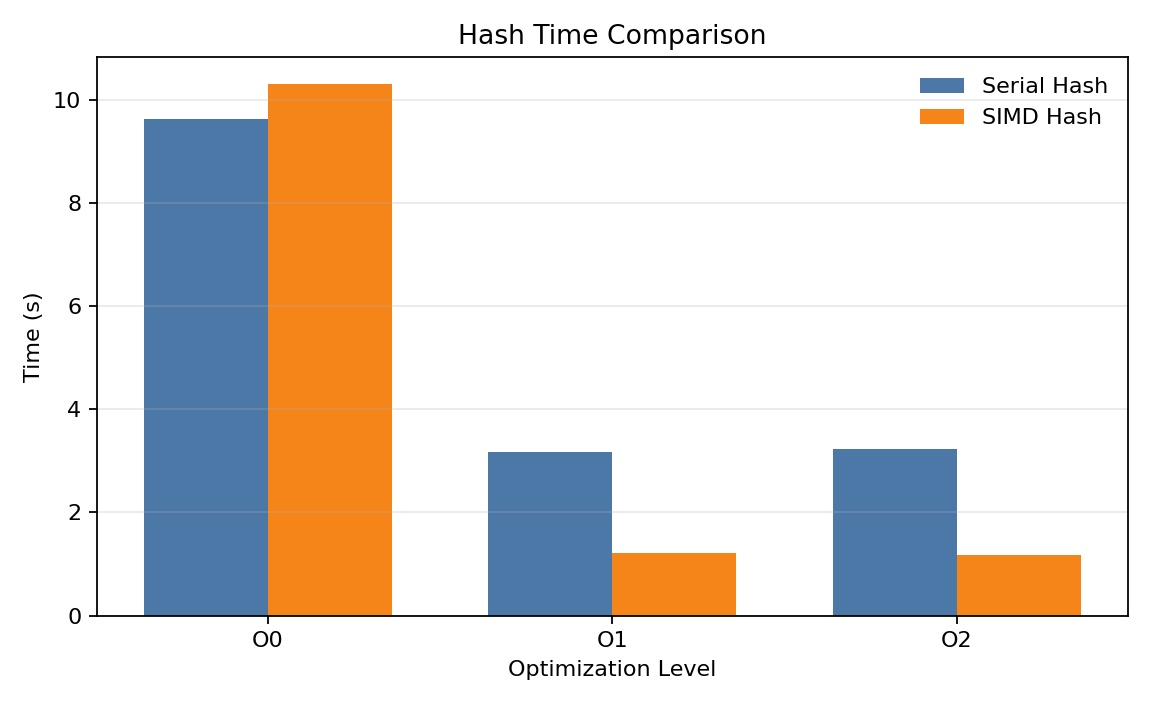
\includegraphics[width=0.82\linewidth]{figures/hash_time.png}
    \caption{不同编译优化等级下的 Hash time 对比}
    \label{fig:hash-time}
\end{figure}

其中 Hash 加速比定义为串行 Hash time 除以 SIMD Hash time。本文所有运行时间对比表均只比较 Hash 阶段，不把候选生成和训练时间计入加速比。

\begin{figure}[H]
    \centering
    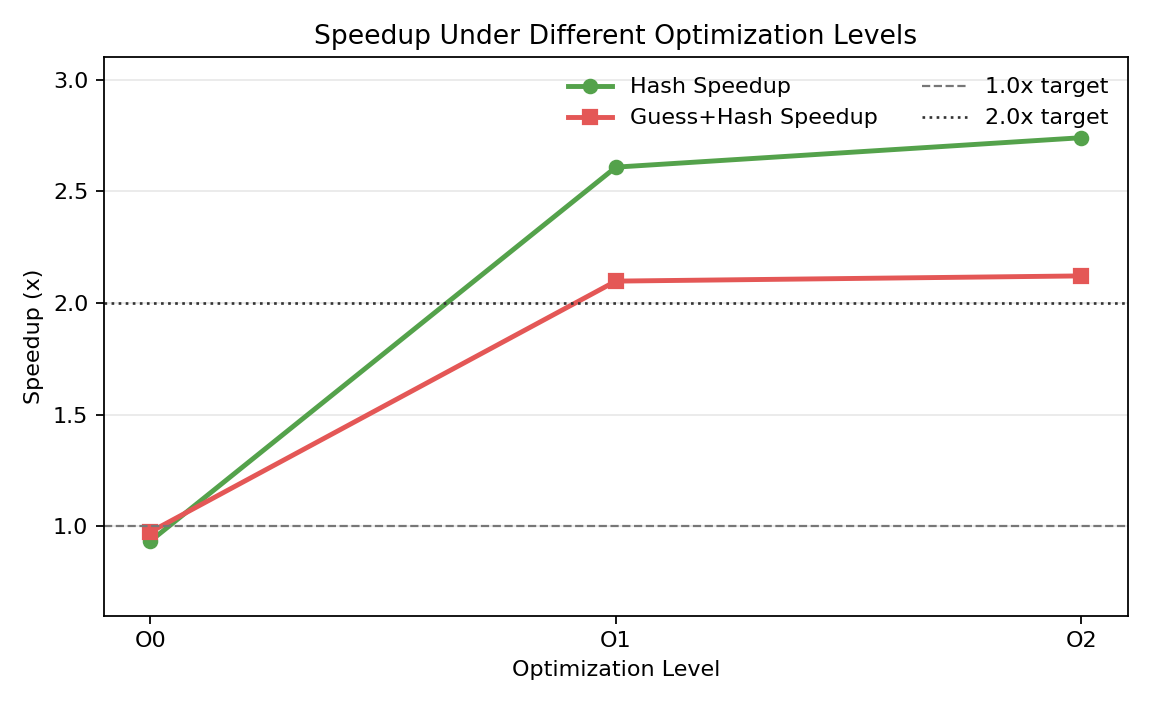
\includegraphics[width=0.82\linewidth]{figures/speedup.png}
    \caption{不同编译优化等级下的加速比}
    \label{fig:speedup}
\end{figure}

图 \ref{fig:speedup} 中，\texttt{-O1} 和 \texttt{-O2} 的 Hash 加速比均超过 2.0x。\texttt{-O0} 的 Hash 加速比低于 1.0x，说明关闭优化后 SIMD Intrinsics 并不会自动带来收益，必须依赖编译器完成较好的指令选择、寄存器分配和冗余代码消除。

\begin{table}[htbp]
    \centering
    \caption{不同编译优化等级下的 Hash time}
    \small
    \begin{tabular}{lcc}
        \toprule
        选项 & 串行 Hash/s & SIMD Hash/s \\
        \midrule
        \texttt{-O0} & 9.61910 & 10.30533 \\
        \texttt{-O1} & 3.16619 & 1.21392 \\
        \texttt{-O2} & 3.22361 & 1.17647 \\
        \bottomrule
    \end{tabular}
\end{table}

\begin{figure}[H]
    \centering
    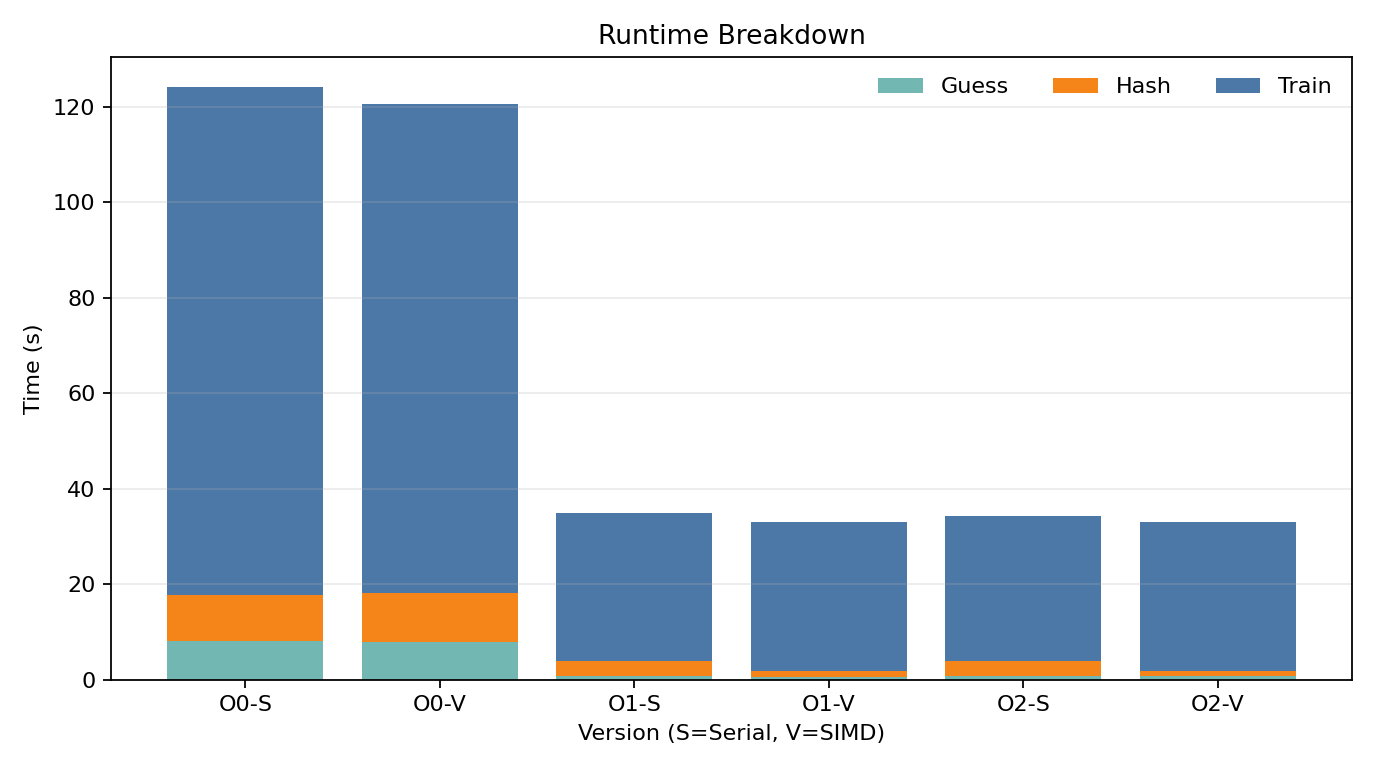
\includegraphics[width=0.88\linewidth]{figures/runtime_breakdown.png}
    \caption{Guess、Hash、Train 三阶段运行时间分解}
    \label{fig:runtime-breakdown}
\end{figure}


从图 \ref{fig:runtime-breakdown} 可以看出：

\begin{itemize}
    \item \texttt{-O1} 下 SIMD 的 Hash 加速比为 2.6082，超过 2.0x。
    \item \texttt{-O2} 下 SIMD 的 Hash 加速比为 2.7401，达到 2.0x 以上。
    \item \texttt{-O0} 下 SIMD 的 Hash time 为 10.30533s，慢于串行版本的 9.61910s，说明在关闭编译优化后，NEON Intrinsics 展开后的寄存器调度、临时变量保存和函数边界开销仍然较重。后续仍将把 \texttt{-O0} 纳入 perf 和汇编对照，用于解释未达标原因；只是本阶段不继续投入代码优化来提高 \texttt{-O0} 加速比。
\end{itemize}

\section{达标加速比（进阶要求）}

当前实验生成候选口令数量约为 $10^7$。为保持数据口径一致，本文统一采用 \path{data/perf_results} 中三次重复运行的均值；旧历史数据不再作为实验结论使用。\texttt{-O2} 下的 Hash time 如下：

\begin{table}[htbp]
    \centering
    \caption{当前 advanced 版本 \texttt{-O2} Hash time}
    \begin{tabular}{lc}
        \toprule
        版本 & Hash time / s \\
        \midrule
        串行对照 & 3.22361 \\
        SIMD 版本 & 1.17647 \\
        \bottomrule
    \end{tabular}
\end{table}

Hash 阶段加速比为：

\[
S_{\text{hash}}=\frac{3.22361}{1.17647}=2.7401.
\]

\begin{table}[htbp]
    \centering
    \caption{进阶目标完成情况}
    \begin{tabular}{lccc}
        \toprule
        编译选项 & 目标加速比 & 实测 Hash 加速比 & 是否达标 \\
        \midrule
        \texttt{-O0} & $>1.0$ & 0.9334 & 暂未达标 \\
        \texttt{-O1} & $\ge 2.0$ & 2.6082 & 达标 \\
        \texttt{-O2} & $\ge 2.0$ & 2.7401 & 达标 \\
        \bottomrule
    \end{tabular}
\end{table}

\section{perf 基础分析（基础要求）}

本节记录 \texttt{perf stat} 的基础性能计数。根据 Linux perf 文档，\texttt{perf stat} 会运行目标命令并汇总硬件/软件性能计数器，因此适合比较串行版本和 SIMD 版本的 cycles、instructions 和 IPC。\footnote{\url{https://man7.org/linux/man-pages/man1/perf-stat.1.html}} 实验使用如下命令采集性能数据，结果保存在 \path{data/perf_results/*_perf.txt} 中：

\begin{lstlisting}[style=cppstyle,caption={perf stat 采集命令},language=bash]
perf stat -r 3 -e cycles,instructions,branches,branch-misses,cache-references,cache-misses ./main_O2
\end{lstlisting}

采集 \texttt{-O0}/\texttt{-O1} 时将二进制名替换为 \texttt{main\_O0}/\texttt{main\_O1}。服务器上 \texttt{branches:u} 事件返回 \texttt{<not supported>}，因此表中不列分支总数；\texttt{branch-misses}、cache 事件、cycles 和 instructions 均正常记录。

\begin{table}[htbp]
    \centering
    \caption{perf stat 统计结果（三次运行均值）}
    \scriptsize
    \begin{tabular}{lcccccc}
        \toprule
        版本 & cycles & instructions & IPC & branch-misses & cache miss率 & elapsed/s \\
        \midrule
        串行 \texttt{-O0} & 3.457e11 & 3.560e11 & 1.03 & 1.022e9 & 0.609\% & 135.16 \\
        SIMD \texttt{-O0} & 3.360e11 & 3.365e11 & 1.00 & 9.827e8 & 0.605\% & 131.444 \\
        串行 \texttt{-O1} & 1.007e11 & 6.029e10 & 0.60 & 6.526e8 & 4.454\% & 39.751 \\
        SIMD \texttt{-O1} & 9.542e10 & 4.717e10 & 0.49 & 6.413e8 & 5.109\% & 37.585 \\
        串行 \texttt{-O2} & 9.860e10 & 5.578e10 & 0.57 & 6.538e8 & 5.539\% & 38.845 \\
        SIMD \texttt{-O2} & 9.564e10 & 4.313e10 & 0.45 & 6.524e8 & 6.776\% & 37.772 \\
        \bottomrule
    \end{tabular}
\end{table}

从基础计数可以得到三个结论。第一，编译优化对总指令数影响非常明显：串行版本从 \texttt{-O0} 的 $3.560\times 10^{11}$ 条指令降到 \texttt{-O2} 的 $5.578\times 10^{10}$ 条，SIMD 版本也从 $3.365\times 10^{11}$ 条降到 $4.313\times 10^{10}$ 条。第二，在 \texttt{-O1}/\texttt{-O2} 下，SIMD 版本的总指令数均低于串行版本，说明 4 路并行确实减少了每个候选口令平均承担的 MD5 计算指令。第三，整程序 elapsed time 的改善小于 Hash time 改善，因为 \texttt{perf stat} 统计的是完整程序，训练和排序阶段仍占用了大量时间。

进一步比较串行和 SIMD 的指令数可知，\texttt{-O1} 下 SIMD 版本比串行版本少约 21.8\% 的指令，\texttt{-O2} 下少约 22.7\% 的指令。这个比例小于 Hash 阶段 2.6x--2.7x 的加速比，原因是 perf 统计覆盖完整程序，训练、排序、候选生成等非 SIMD 部分仍会贡献大量指令。换言之，\texttt{perf stat} 反映的是整程序视角，而 Hash time 反映的是被优化函数所在阶段的局部视角，两者并不矛盾。

\section{perf 进阶分析（进阶要求）}

在基础计数之外，本实验使用 \texttt{perf record} 采集 SIMD 版本调用栈样本，并用 \texttt{perf report} 查看热点函数；随后用 \texttt{objdump} 检查编译器是否将 C++/NEON Intrinsics 转换成预期的 NEON 汇编。\footnote{\url{https://man7.org/linux/man-pages/man1/perf-record.1.html}} 由于前文已经说明串行版本难以获得稳定、集中的 MD5 热点，本节热点分析只针对 SIMD 版本展开；串行版本保留 \texttt{perf stat} 作为对照。

\begin{lstlisting}[style=cppstyle,caption={热点和汇编分析命令},language=bash]
perf record -g ./main
perf report --stdio > perf_report.txt
objdump -d main > main.asm
\end{lstlisting}

\subsection{热点函数}

\texttt{perf report} 输出均位于 \path{data/perf_results} 目录，对应文件分别为 \path{O0_simd_report.txt}、\path{O1_simd_report.txt} 和 \path{O2_simd_report.txt}。主要热点如下：

\begin{table}[htbp]
    \centering
    \caption{SIMD 版本 perf report 主要热点}
    \small
    \begin{tabular}{lcccc}
        \toprule
        版本 & \texttt{model::train} & \texttt{model::order} & \texttt{segment::order} & \texttt{MD5Hash\_simdversion} \\
        \midrule
        \texttt{-O0} & 54.86\% & 23.06\% & 15.82\% & 7.71\% \\
        \texttt{-O1} & 53.46\% & 20.89\% & 20.73\% & 3.66\% \\
        \texttt{-O2} & 54.34\% & 20.54\% & 19.43\% & 2.75\% \\
        \bottomrule
    \end{tabular}
\end{table}

\begin{figure}[H]
    \centering
    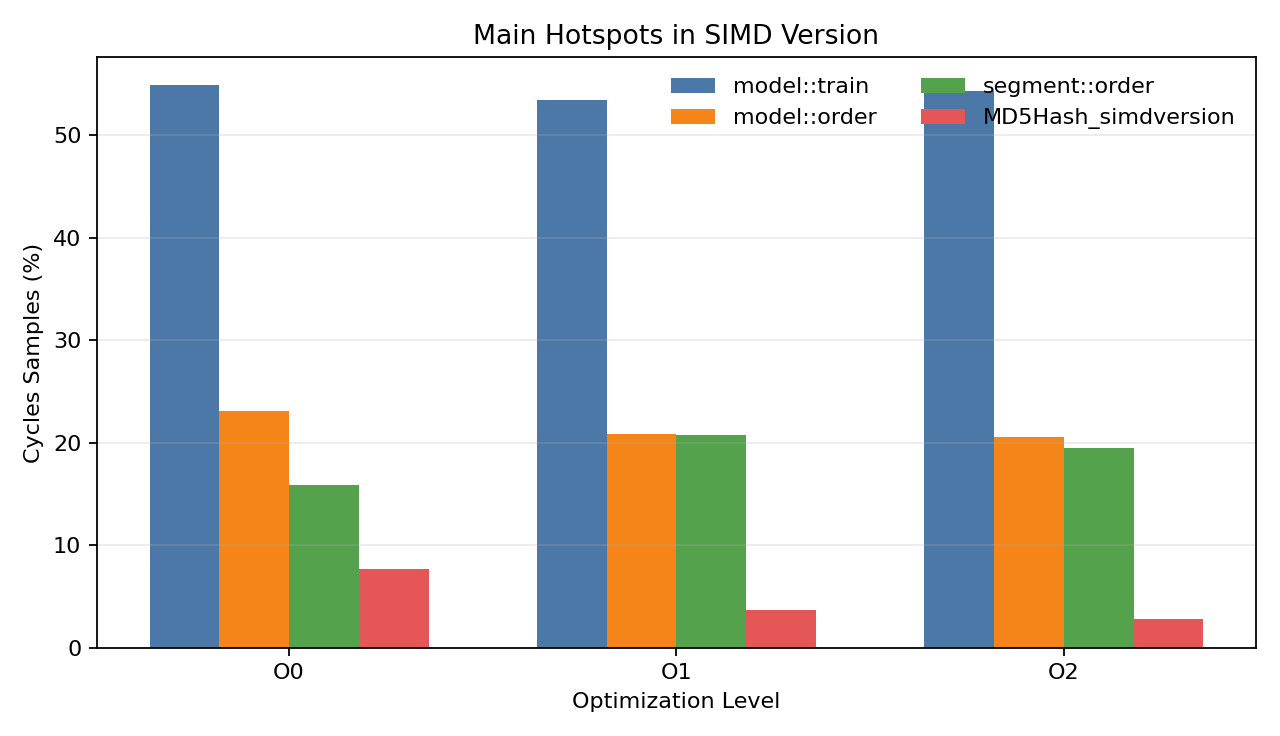
\includegraphics[width=0.86\linewidth]{figures/perf_hotspots.png}
    \caption{SIMD 版本主要热点占比}
    \label{fig:perf-hotspots}
\end{figure}

这个结果说明整程序热点主要集中在 PCFG 训练、模式统计和排序上，而不是 MD5 本身。其原因是 \texttt{perf record} 采样的是完整程序，训练阶段需要读取、解析和统计大量口令，\texttt{model::order}/\texttt{segment::order} 内部又包含大量排序和字符串比较。因此即使 Hash 阶段已经通过 SIMD 获得 2x 以上加速，在整程序热点图中 \texttt{MD5Hash\_simdversion} 仍只占较小比例。

从图 \ref{fig:perf-hotspots} 可以看到，\texttt{model::train} 在三个优化等级下都稳定占据约 53\%--55\% 的采样比例，说明训练逻辑是整程序最主要的固定开销。\texttt{MD5Hash\_simdversion} 的占比从 \texttt{-O0} 的 7.71\% 降到 \texttt{-O2} 的 2.75\%，一方面是因为编译优化显著减少了 MD5 相关指令，另一方面也说明 Hash 阶段优化后在完整程序中的权重下降。此时继续只优化 MD5 的边际收益会逐渐变小。

\subsection{编译选项与汇编}

反汇编结果均位于 \path{data/perf_results} 目录，对应文件分别为 \path{O0_simd_main.asm}、\path{O1_simd_main.asm} 和 \path{O2_simd_main.asm}。三个文件均可定位到 \texttt{MD5Hash\_simdversion} 符号，说明 SIMD MD5 没有被错误替换为纯串行实现。\texttt{-O1}/\texttt{-O2} 下反汇编中可以观察到以 NEON 向量寄存器为操作对象的加法、异或、或、移位和访存指令，对应 C++ 代码中的 \texttt{vaddq\_u32}、\texttt{veorq\_u32}、\texttt{vorrq\_u32}、\texttt{vshlq\_n\_u32}/\texttt{vshrq\_n\_u32} 以及 \texttt{vld1q\_u32} 等 Intrinsics。

\begin{lstlisting}[style=cppstyle,caption={\texttt{-O2} 下 \texttt{MD5Hash\_simdversion} 的部分 NEON 汇编}]
411114: add  v0.4s,  v7.4s,  v0.4s
411124: shl  v3.4s,  v0.4s,  #7
411128: ushr v0.4s,  v0.4s,  #25
411138: orr  v0.16b, v3.16b, v0.16b
411168: eor  v1.16b, v1.16b, v10.16b
411190: shl  v2.4s,  v1.4s,  #12
411194: ushr v1.4s,  v1.4s,  #20
4111a4: orr  v2.16b, v2.16b, v1.16b
\end{lstlisting}

其中 \texttt{add v?.4s} 表示 4 个 32-bit lane 同时加法，\texttt{eor}/\texttt{orr} 对应 MD5 轮函数中的按位逻辑运算，\texttt{shl + ushr + orr} 组合对应循环左移。这说明编译器确实将 NEON Intrinsics 降低为向量汇编指令，而不是展开为 4 次独立的标量 MD5。

从性能计数和汇编规模看，\texttt{-O0} 下 SIMD 版本仍有较重开销。其反汇编文件约 1.61 MB，而 \texttt{-O1}/\texttt{-O2} 分别约 0.98 MB 和 0.92 MB；同时 \texttt{-O0} SIMD 的总指令数为 $3.365\times 10^{11}$，远高于 \texttt{-O2} SIMD 的 $4.313\times 10^{10}$。这说明 \texttt{-O0} 没有充分进行函数内联、寄存器分配和冗余代码消除，导致 SIMD 计算节省下来的数据并行收益被额外指令和访存开销抵消。因此 \texttt{-O0} Hash 加速比只有 0.9334，未达到 1.0x。

\texttt{-O1}/\texttt{-O2} 下，编译器能更好地优化 NEON Intrinsics 生成的机器码。与串行版本相比，\texttt{-O1} SIMD 指令数从 $6.029\times 10^{10}$ 降至 $4.717\times 10^{10}$，\texttt{-O2} SIMD 指令数从 $5.578\times 10^{10}$ 降至 $4.313\times 10^{10}$；配合 4 路 lane 并行，Hash 阶段分别达到 2.6082x 和 2.7401x。短口令 fast path 还减少了 \texttt{StringProcess}、动态分配和内存初始化开销，使热点进一步集中到真正的 MD5 轮函数计算上。


\end{document}
